\documentclass[10pt,a4paper]{article}
\usepackage[singlespacing, onehalfspacing]{setspace}
\usepackage{parskip}
\usepackage[spaces,hyphens]{url}
\usepackage{enumitem}
\usepackage[left=3cm,right=3cm,top=3cm,bottom=3cm]{geometry}
\usepackage{titlesec}
\usepackage{fancyhdr}
\usepackage{tocloft}
\usepackage{longtable}
\usepackage{tabularx}
\usepackage{booktabs}
\usepackage{caption}
\usepackage{amsmath}
\usepackage{amssymb}
\usepackage{colortbl}
\usepackage{tikz}
\usepackage{pgfplots}
\usepackage{pdflscape}
\usepackage{pbox}
\usepackage{dcolumn}
\usepackage[figuresleft]{rotating}
\usepackage{subcaption}
\usepackage{tcolorbox}
\usepackage{listings}
\usepackage[export]{adjustbox}

\usepackage[backend=biber, style=authoryear-comp, sorting=nyt, url=false, isbn=false, doi=false, clearlang=false, maxbibnames=10, maxcitenames=2]{biblatex}
\addbibresource{../library.bib}

\pgfplotsset{compat=1.17}

\usepackage[colorlinks = true,
            linkcolor = PN1,
            urlcolor  = F3,
            citecolor = F3,
            anchorcolor = A4]{hyperref}

% - Polar Night
\definecolor{PN0}{RGB}{64,52,64}
\definecolor{PN1}{RGB}{59,66,82}
\definecolor{PN2}{RGB}{67,76,94}
\definecolor{PN3}{RGB}{76,86,106}

% - Snow Storm
\definecolor{SS0}{RGB}{216,222,233}
\definecolor{SS1}{RGB}{229,233,240}
\definecolor{SS2}{RGB}{236,239,244}

% - Frost
\definecolor{F0}{RGB}{143,188,187}
\definecolor{F1}{RGB}{136,192,208}
\definecolor{F2}{RGB}{129,161,193}
\definecolor{F3}{RGB}{94,129,172}

% - Aurora
\definecolor{A0}{RGB}{191,97,106}
\definecolor{A1}{RGB}{208,135,112}
\definecolor{A2}{RGB}{235,203,139}
\definecolor{A3}{RGB}{163,190,140}
\definecolor{A4}{RGB}{180,142,173}

\definecolor{light-gray}{gray}{0.95}

\lstset{language=R,
    basicstyle=\fontsize{6}{9}\selectfont\ttfamily,
    backgroundcolor = \color{light-gray},
    %stringstyle=\color{F3},
    %otherkeywords={0,1,2,3,4,5,6,7,8,9},
    %morekeywords={TRUE,FALSE},
    deletekeywords={data,frame,length,as,character},
    %keywordstyle=\color{A1},
    commentstyle=\color{PN3},
    showstringspaces=false,
    rulecolor=\color{black},
    frameshape={RYR}{Y}{Y}{RYR}
}

\widowpenalty90000
\clubpenalty90000

\pagestyle{fancy}
\setlength{\headheight}{15pt}
\fancyhf{}
\fancyhead[R]{\thepage}
\fancyhead[L]{\textit{Data Science 101 -- Regressionen}}
\titleformat*{\section}{\large\bfseries}
\renewcommand\cftsecfont{\normalsize}
\renewcommand\cftsecpagefont{\footnotesize\bfseries}
\renewcommand{\cftsecleader}{\cftdotfill{\cftdotsep}}
\setlength{\cftbeforesecskip}{-2pt}
\renewcommand{\abstractname}{}

\makeatletter
\setlength{\@fptop}{0pt}
\setlength{\parskip}{0.5pt}
\makeatother

\renewcommand{\contentsname}{Übersicht}

\begin{document}

\thispagestyle{empty}
\frenchspacing
\begin{flushleft}
\begin{tabular}{p{11.5cm} r}
Martin Kerntopf & 25. Januar 2022 \\
Email: martin.kerntopf@uni-greifswald.de \\
Seminar: Data Science für Geistes- und Sozialwissenschaftler 
\end{tabular}
\end{flushleft}
\hrule
\begin{center}
\vspace{0.4cm}
\large{\textsc{Regressionen}}

\vspace{0.4cm}
\end{center}
%\vspace{-0.2cm}
\hrule 
%\vspace{0.2cm}
\frenchspacing

\tableofcontents

\section{Einleitung}
    \subsection{Relevanz}
\section{Theorie}
    \subsection{Grundlagen}
    \subsection{Annahmen}
        \subsubsection{Der Erwartungswert der Residuen ist Null}
        Die erste Annahme geht davon aus, dass die Fehlerterme im Durchschnitt Null ergeben (genannt Erwartungswert). Es gibt sowohl Abweichungen gegen unten als auch gegen oben. Im Schnitt heben sich diese jedoch auf. Deshalb werden auch die Quadratterme der Residuen minimiert und nicht die Residuen selber, da bei Quadratwerten sich negative und positive Abweichungen nicht aufheben.
        \subsubsection{Fehlerterme sind unkorreliert}
        Die zweite Annahme ist eine sehr wichtige Annahme. Sie besagt, dass die Residuen nicht miteinander korrelieren. Dies tun sie dann, wenn wichtige Variablen nicht ins Modell aufgenommen wurden.

        \subsubsection{Homo- und Heteroskedastizität}
        Die Homoskedastizität besagt, dass die Varianz der Fehlerterme gleichmässig verteilt ist. Ist dies nicht der Fall spricht man von Heteroskedastizität. Liegt Heteroskedastizität vor, ist OLS nicht mehr effizient und es müssen andere Verfahren angewandt werden.

        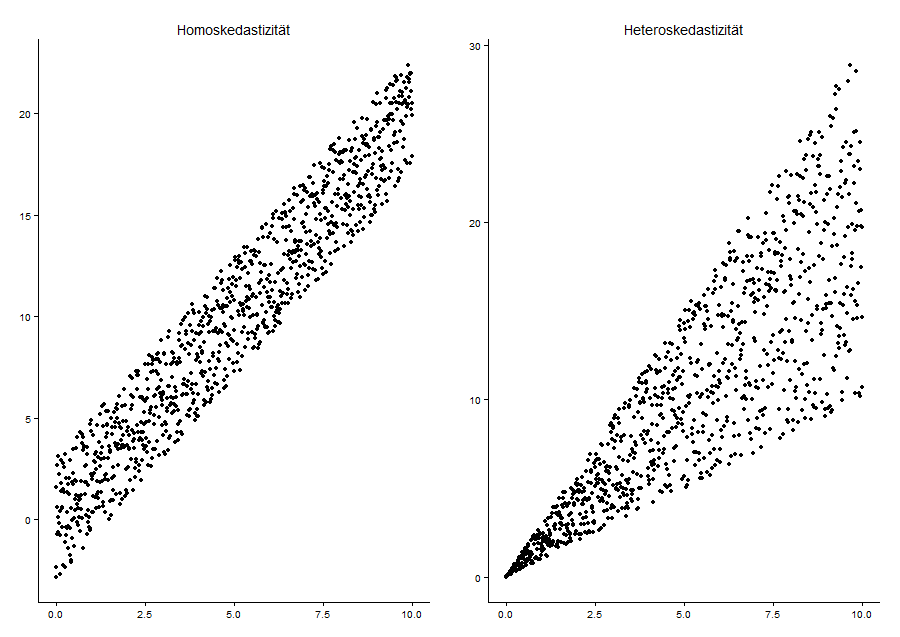
\includegraphics[max width=\textwidth]{../Plots/homo_heterosked.png}

        \subsubsection{Fehlerterme sind normalverteilt}
        Die Normalverteilung (auch Gauss-Verteilung genannt) ist eine stetige Verteilung. Viele Fehler lassen sich durch diese symmetrische Verteilung erklären.

        
    \subsection{Regressionsformen}
\section{Praxis}
    \subsection{Modell}
    \subsection{Ergebnistabelle}
    \subsection{Plotten}
    \subsection{Erweiterte Darstellung}

\section{Weiterführende Literatur}
\begin{itemize}
    \item \fullcite{Hedderich2016} 
    \item \fullcite{Wolf2010}
    \item \fullcite{Ciaburro2018}
    \item \fullcite{Pardoe2020}
  \end{itemize}
\end{document}